%%%%%%%%%%%%%%%%%%%%%%%%%%%%%%%%%%%%%%%%%
% Programming/Coding Assignment
% LaTeX Template
%
% This template has been downloaded from:
% http://www.latextemplates.com
%
% Original author:
% Ted Pavlic (http://www.tedpavlic.com)
%
% Note:
% The \lipsum[#] commands throughout this template generate dummy text
% to fill the template out. These commands should all be removed when 
% writing assignment content.
%
% This template uses a Perl script as an example snippet of code, most other
% languages are also usable. Configure them in the "CODE INCLUSION 
% CONFIGURATION" section.
%
%%%%%%%%%%%%%%%%%%%%%%%%%%%%%%%%%%%%%%%%%

%----------------------------------------------------------------------------------------
%	PACKAGES AND OTHER DOCUMENT CONFIGURATIONS
%----------------------------------------------------------------------------------------

\documentclass{article}

\usepackage{fancyhdr} % Required for custom headers
\usepackage{lastpage} % Required to determine the last page for the footer
\usepackage{extramarks} % Required for headers and footers
\usepackage[usenames,dvipsnames]{color} % Required for custom colors
\usepackage{graphicx} % Required to insert images
\usepackage{listings} % Required for insertion of code
\usepackage{courier} % Required for the courier font
\usepackage{lipsum} % Used for inserting dummy 'Lorem ipsum' text into the template
\usepackage{setspace}
\usepackage{color}
\usepackage{comment}
\usepackage{caption}

\usepackage{hyperref}
\usepackage{natbib}
\usepackage{underscore}

\hypersetup{
    colorlinks=true,
    linkcolor=blue,
    filecolor=magenta,      
    urlcolor=cyan,
    breaklinks=true
}

%\usepackage[]{algorithm2e}
\usepackage{pdfpages}




%For python inclusion (http://widerin.org/blog/syntax-highlighting-for-python-scripts-in-latex-documents)
\definecolor{Code}{rgb}{0,0,0}
\definecolor{Decorators}{rgb}{0.5,0.5,0.5}
\definecolor{Numbers}{rgb}{0.5,0,0}
\definecolor{MatchingBrackets}{rgb}{0.25,0.5,0.5}
\definecolor{Keywords}{rgb}{0,0,1}
\definecolor{self}{rgb}{0,0,0}
\definecolor{Strings}{rgb}{0,0.63,0}
\definecolor{Comments}{rgb}{0,0.63,1}
\definecolor{Backquotes}{rgb}{0,0,0}
\definecolor{Classname}{rgb}{0,0,0}
\definecolor{FunctionName}{rgb}{0,0,0}
\definecolor{Operators}{rgb}{0,0,0}
\definecolor{Background}{rgb}{0.98,0.98,0.98}

% Margins
\topmargin=-0.45in
\evensidemargin=0in
\oddsidemargin=0in
\textwidth=6.5in
\textheight=9.0in
\headsep=0.25in

\linespread{1.1} % Line spacing

% Set up the header and footer
\pagestyle{fancy}
\lhead{\hmwkAuthorName} % Top left header
%\chead{\hmwkClass\ (\hmwkClassInstructor\ \hmwkClassTime): \hmwkTitle} % Top center head
\chead{\hmwkClass\ (\hmwkClassInstructor): \hmwkTitle} % Top center head
\rhead{\firstxmark} % Top right header
\lfoot{\lastxmark} % Bottom left footer
\cfoot{} % Bottom center footer
\rfoot{Page\ \thepage\ of\ \protect\pageref{LastPage}} % Bottom right footer
\renewcommand\headrulewidth{0.4pt} % Size of the header rule
\renewcommand\footrulewidth{0.4pt} % Size of the footer rule

\setlength\parindent{0pt} % Removes all indentation from paragraphs

%----------------------------------------------------------------------------------------
%	CODE INCLUSION CONFIGURATION
%----------------------------------------------------------------------------------------

\definecolor{MyDarkGreen}{rgb}{0.0,0.4,0.0} % This is the color used for comments
\lstloadlanguages{Perl} % Load Perl syntax for listings, for a list of other languages supported see: ftp://ftp.tex.ac.uk/tex-archive/macros/latex/contrib/listings/listings.pdf
\lstset{language=Perl, % Use Perl in this example
        frame=single, % Single frame around code
        basicstyle=\small\ttfamily, % Use small true type font
        keywordstyle=[1]\color{Blue}\bf, % Perl functions bold and blue
        keywordstyle=[2]\color{Purple}, % Perl function arguments purple
        keywordstyle=[3]\color{Blue}\underbar, % Custom functions underlined and blue
        identifierstyle=, % Nothing special about identifiers                                         
        commentstyle=\usefont{T1}{pcr}{m}{sl}\color{MyDarkGreen}\small, % Comments small dark green courier font
        stringstyle=\color{Purple}, % Strings are purple
        showstringspaces=false, % Don't put marks in string spaces
        tabsize=5, % 5 spaces per tab
        %
        % Put standard Perl functions not included in the default language here
        morekeywords={rand},
        %
        % Put Perl function parameters here
        morekeywords=[2]{on, off, interp},
        %
        % Put user defined functions here
        morekeywords=[3]{test},
       	%
        morecomment=[l][\color{Blue}]{...}, % Line continuation (...) like blue comment
        numbers=left, % Line numbers on left
        firstnumber=1, % Line numbers start with line 1
        numberstyle=\tiny\color{Blue}, % Line numbers are blue and small
        stepnumber=5 % Line numbers go in steps of 5
}

% Creates a new command to include a perl script, the first parameter is the filename of the script (without .pl), the second parameter is the caption
\newcommand{\perlscript}[2]{
\begin{itemize}
\item[]\lstinputlisting[caption=#2,label=#1]{#1.pl}
\end{itemize}
}


%----------------------------------------------------------------------------------------
%	DOCUMENT STRUCTURE COMMANDS
%	Skip this unless you know what you're doing
%----------------------------------------------------------------------------------------

% Header and footer for when a page split occurs within a problem environment
\newcommand{\enterProblemHeader}[1]{
\nobreak\extramarks{#1}{#1 continued on next page\ldots}\nobreak
\nobreak\extramarks{#1 (continued)}{#1 continued on next page\ldots}\nobreak
}

% Header and footer for when a page split occurs between problem environments
\newcommand{\exitProblemHeader}[1]{
\nobreak\extramarks{#1 (continued)}{#1 continued on next page\ldots}\nobreak
\nobreak\extramarks{#1}{}\nobreak
}

\setcounter{secnumdepth}{0} % Removes default section numbers
\newcounter{homeworkProblemCounter} % Creates a counter to keep track of the number of problems

\newcommand{\homeworkProblemName}{}
\newenvironment{homeworkProblem}[1][Problem \arabic{homeworkProblemCounter}]{ % Makes a new environment called homeworkProblem which takes 1 argument (custom name) but the default is "Problem #"
\stepcounter{homeworkProblemCounter} % Increase counter for number of problems
\renewcommand{\homeworkProblemName}{#1} % Assign \homeworkProblemName the name of the problem
\section{\homeworkProblemName} % Make a section in the document with the custom problem count
\enterProblemHeader{\homeworkProblemName} % Header and footer within the environment
}{
\exitProblemHeader{\homeworkProblemName} % Header and footer after the environment
}

\newcommand{\problemAnswer}[1]{ % Defines the problem answer command with the content as the only argument
\noindent\framebox[\columnwidth][c]{\begin{minipage}{0.98\columnwidth}#1\end{minipage}} % Makes the box around the problem answer and puts the content inside
}

\newcommand{\homeworkSectionName}{}
\newenvironment{homeworkSection}[1]{ % New environment for sections within homework problems, takes 1 argument - the name of the section
\renewcommand{\homeworkSectionName}{#1} % Assign \homeworkSectionName to the name of the section from the environment argument
\subsection{\homeworkSectionName} % Make a subsection with the custom name of the subsection
\enterProblemHeader{\homeworkProblemName\ [\homeworkSectionName]} % Header and footer within the environment
}{
\enterProblemHeader{\homeworkProblemName} % Header and footer after the environment
}

%----------------------------------------------------------------------------------------
%	NAME AND CLASS SECTION
%----------------------------------------------------------------------------------------

\newcommand{\hmwkTitle}{Assignment\ \#3 } % Assignment title
%\newcommand{\hmwkDueDate}{Monday,\ January\ 1,\ 2012} % Due date
\newcommand{\hmwkClass}{Introduction to Web Science} % Course/class
%\newcommand{\hmwkClassTime}{10:30am} % Class/lecture time
\newcommand{\hmwkClassInstructor}{Dr. Nelson} % Teacher/lecturer
\newcommand{\hmwkAuthorName}{Alexander Nwala} % Your name

%----------------------------------------------------------------------------------------
%	TITLE PAGE
%----------------------------------------------------------------------------------------

\title{
\vspace{2in}
\textmd{\textbf{\hmwkClass:\ \hmwkTitle}}\\
%\normalsize\vspace{0.1in}\small{Due\ on\ \hmwkDueDate}\\
%\vspace{0.1in}\large{\textit{\hmwkClassInstructor\ \hmwkClassTime}}
\vspace{0.1in}\large{\textit{\hmwkClassInstructor}}
\vspace{3in}
}

\author{\textbf{\hmwkAuthorName}}
\date{Thursday, April 2, 2015} % Insert date here if you want it to appear below your name

%----------------------------------------------------------------------------------------

\begin{document}

\maketitle



%----------------------------------------------------------------------------------------
%	TABLE OF CONTENTS
%----------------------------------------------------------------------------------------

%\setcounter{tocdepth}{1} % Uncomment this line if you don't want subsections listed in the ToC

\newpage
\tableofcontents
\newpage

%----------------------------------------------------------------------------------------
%	PROBLEM 1
%----------------------------------------------------------------------------------------

% To have just one problem per page, simply put a \clearpage after each problem

\begin{homeworkProblem}
For the text you saved for the 10000 URIs from A1, Q2:
Use the ``boilerpipe'' software to remove the HTML templates from all HTML pages (document how many pages link from the tweets were non-HTML and had to be skipped)\\

\url{https://code.google.com/p/boilerpipe/}\\
WSDM 2010 paper:
\url{http://www.l3s.de/~kohlschuetter/boilerplate/}\\

For how many of the 10000 URIs was boilerpipe successful? 
Compare the total words, unique words, and byte sizes before and after use of boilerpipe.
For what classes of pages was it successful?  
For what classes of pages was it unsuccessful?
Provide examples of both successful and unsuccessful removals and discuss at length.\\

%\lstinputlisting[breaklines=true, caption=Curl Demo]{"/home/anwala/CS 895/Assignment 1/problem1_curlDemonstration.py"}
%\lstinputlisting[breaklines=true, caption=Hash function; extract HTML funtion; and strip HTML tags function]{hashExtractProcessHTMlSnippet.py}


\begin{comment}
\begin{figure}
    \caption{curlDemoOutput}
    \begin{center}
        \includegraphics{curlDemo} % Example image
    \end{center}
\end{figure}
\end{comment}

%\problemAnswer
%{
    


    \textbf{SOLUTION 1}\\

    The solution for this problem is outlined by the following steps:\\

    \textbf{Remove boilerplate from HTML pages:}
    Due to Listing 1, the HTML templates derived after dereferencing the URIs were removed with justtext \cite{justText}\\

    \lstinputlisting[breaklines=true, caption=Remove Boilerplate]{removeBoilerplateSnippet.py}

    Consider the following remarks:
    Given the list of 10,000 URIs, only 2,164 were unique URIs from A2 - I believe this was caused due to overlap in my search results from Twitter (in retrospect, my algorithm to retrieve URIs should not have used search).\\

    Given my initial list of 2,164 URIs, 1,132 were skipped due to ERRORs ranging from 404s to corrupt URIs as seen by the following examples of HTTP response codes:
    \begin{verbatim}

    $ curl -I https://api.twitter.com/oauth/authorize?oauth_token
    =8bwrg25dbghw8aszsfc0wul3q6gxswey
    HTTP/1.1 403 Forbidden

    $ curl -I http://click.linksynergy.com/link?id=vdg03e6l9pw&offerid=
    210072.9001235091&type=2&murl=
    http://www.animate-onlineshop.jp/products/detail.php%3fproduct_id%3d1235091
    HTTP/1.1 400 Bad Request

    $ curl -I http://p0p.pw/erh
    HTTP/1.1 404 Not Found

    $ curl -I http://raumu.ciao.jp/yyc/
    HTTP/1.1 404 Not Found

    $ curl -I http://butta.info/u1f3rd/
    curl: (6) Could not resolve host: butta.info

    \end{verbatim}

    There were 60 successful text extraction operations from the list of URIs.\\

    Because of the low success rate, I began investigating a possible cause by randomly sampling 15 URIs. I consider the following results below, a justification for the low success rate.

    \begin{verbatim}

    5 URIs: links of Google sites with no content which required a 
    click to redirect
    5 URIs: Japanese sites ranging from blogs to sites with no content
    3 URIs: 2 Spanish news sites which required clicks to see content,
    1 Facebook site
    2 URIs: 1 image and one was unavailable (404)

    \end{verbatim}

    Consider the following statistic collected from 60 successful text extraction operations:

    \begin{verbatim}
    Total words before removal: 549,788
    Total words after removal: 31,135

    Total unique words before removal: 51,044
    Total unique words after removal: 7,819

    Total size (bytes) before removal: 31,010,041
    Total size (bytes) after removal: 192,437
    \end{verbatim}

    The classes of pages for which boilerplate removal was successful includes: organized pages with well defined/extensive text areas such as blogs and pages with comment sections. Overall, pages in which the template was on the left and right with text in the middle were successfull. Consider the following examples (charts 1 - 3) of successful removals (green boxes) based on the format described.


    \begin{verbatim}

    Chart Example 1 URI:
    https://www-304.ibm.com/connections/blogs/socialbusiness/
    entry/you_are_sitting_on_a_volcano_that_is_ready_to_blow?lang=en_us

    Chart Example 2 URI
    http://www.thedailybeast.com/articles/2015/02/03/average-
    soldiers-don-t-trust-their-generals-and-they-have-a-point.html

    Chart Example 3 URI
    http://prod.www.giants.clubs.nfl.com/news-and-blogs/article-
    1/know-your-giants-te-larry-donnell-/dbaf4b75-cb7c-40f3-b326-
    22a5600aebbd?utm_source=dlvr.it&utm_medium=twitter

    \end{verbatim}

    \includepdf[pages={1,2,3}]{boilerplate.pdf}
   
    The classes of pages for which boilerplate removal was unsuccessful includes:
    Pages with disorganized format (no well defined template) in which text was spread accross template as well as pages with unconventional layouts: 

    \begin{verbatim}

    Chart Example 4 URI:
    http://www.stocktradepartner.com/

    Chart Example 5 URI:
    http://www.fandango.com/dawnoftheplanetoftheapes_156265/movieo
    verview?wssaffid=11838&wssac=123&cjid=cj_10576763_7644471_

    Chart Example 6 URI:
    http://www.yesasia.com/us/you-who-came-from-the-stars-blu-ray-
    vol-2-japan-version/1037741202-0-0-0-en/info.html

    \end{verbatim}

    \includepdf[pages={4,5,6}]{boilerplate.pdf}

    
    
    
%}



\end{homeworkProblem}

%----------------------------------------------------------------------------------------
%	PROBLEM 2
%----------------------------------------------------------------------------------------

\begin{homeworkProblem}
Collection1: Extract all the unique terms and their frequency from the 10000 files*\\

Collection2: Extract all the unique terms and their frequency of the 10000 files* after running boilerpipe\\

Construct a table with the top 50 terms from each collection. 
Find a common stop word list.  How many of the 50 terms are on that stop word list?\\

For both collections, construct a graph with the x-axis as word rank, and y-axis as word frequency. \\

Do either follow a Zipf distribution? Support your answer.\\

\textbf{SOLUTION 2}\\

The solution for this problem is outlined by the following steps:\\

\textbf{Extract unique terms:} Due to Listing 2, the unique terms were retrieved by splitting the string of all the HTML files on the space character. Subsequently Listing 2. kept track of the term and term frequencies in a dictionary.

\lstinputlisting[breaklines=true, caption=Get Unique Terms]{getUniqueTermsSnippet.py}

\textbf{Construct table:}
Consider Table 1 and 2.\\

\begin{table}
    \caption{Top 50 Terms Extracted From HTML Files} % title of Table
    \centering % used for centering table
    \begin{tabular}{c | c | c} % centered columns (4 columns)
    \hline\hline %inserts double horizontal lines
    Item & Term & Frequency \\ [0.5ex] % inserts table 
    %heading
    \hline \hline% inserts single horizontal line
    1 & \textless div & 2924 \\ \hline
    2 & = & 2033 \\ \hline
    3 & the & 1944 \\ \hline
    4 & \textless a & 1819 \\ \hline
    5 & to & 1556 \\ \hline
    6 & and & 1503 \\ \hline
    7 & a & 1247 \\ \hline
    8 & of & 1094 \\ \hline
    9 & \{ & 1085 \\ \hline
    10 & \textless li\textgreater \textless a & 971 \\ \hline
    11 & \textless span & 953 \\ \hline
    12 & \textless/div\textgreater & 871 \\ \hline
    13 & in & 834 \\ \hline
    14 & \{ & 792 \\ \hline
    15 & for & 767 \\ \hline
    16 & - & 692 \\ \hline
    17 & \textless li & 682 \\ \hline
    18 & at & 661 \\ \hline
    19 & var & 579 \\ \hline
    20 & point:false, & 574 \\ \hline
    21 & on & 561 \\ \hline
    22 & + & 557 \\ \hline
    23 & \textless/div\textgreater & 555 \\ \hline
    24 & is & 550 \\ \hline
    25 & target=``_blank'' & 547 \\ \hline
    26 & B & 529 \\ \hline
    27 & position:``left''\}, & 506 \\ \hline
    28 & you & 460 \\ \hline
    29 & your & 459 \\ \hline
    30 & \textless/li\textgreater & 446 \\ \hline
    31 & class=``b-link'' & 442 \\ \hline
    32 & with & 428 \\ \hline
    33 & I & 419 \\ \hline
    34 & blog-admin & 401 \\ \hline
    35 & target='_self' & 400 \\ \hline
    36 & \&amp; & 392 \\ \hline
    37 & 2014 & 389 \\ \hline
    38 & \textless/a\textgreater & 376 \\ \hline
    39 & December & 373 \\ \hline
    40 & 0 & 372 \\ \hline
    41 & rel=``nofollow'' & 368 \\ \hline
    42 & \textless img & 355 \\ \hline
    43 & onclick="return & 352 \\ \hline
    44 & if & 350 \\ \hline
    45 & nofollow:false,tab_target:false, & 348 \\ \hline
    46 & class=``b-ico'' & 337 \\ \hline
    47 & type=``hidden'' & 333 \\ \hline
    48 & The & 322 \\ \hline
    49 & \} & 305 \\ \hline

    50 & class="b-link & 296 \\ [1ex] 
    \hline %inserts single line
    \end{tabular}
    \label{table:nonlin} % is used to refer this table in the text
    \end{table}

    \begin{table}
        \caption{Top 50 Terms Extracted Post Boilerplate Removal} % title of Table
        \centering % used for centering table
        \begin{tabular}{c | c | c} % centered columns (4 columns)
        \hline\hline %inserts double horizontal lines
        Item & Term & Frequency \\ [0.5ex] % inserts table 
        %heading
        \hline \hline% inserts single horizontal line
        1 & the & 1164 \\ \hline
        2 & and & 925 \\ \hline
        3 & to & 899 \\ \hline
        4 & a & 771 \\ \hline
        5 & of & 625 \\ \hline
        6 & in & 500 \\ \hline
        7 & is & 423 \\ \hline
        8 & you & 389 \\ \hline
        9 & I & 379 \\ \hline
        10 & for & 309 \\ \hline
        11 & with & 259 \\ \hline
        12 & that & 258 \\ \hline
        13 & your & 220 \\ \hline
        14 & on & 203 \\ \hline
        15 & was & 184 \\ \hline
        16 & are & 183 \\ \hline
        17 & or & 170 \\ \hline
        18 & it & 153 \\ \hline
        19 & at & 150 \\ \hline
        20 & be & 150 \\ \hline
        21 & as & 146 \\ \hline
        22 & this & 140 \\ \hline
        23 & by & 137 \\ \hline
        24 & will & 130 \\ \hline
        25 & have & 120 \\ \hline
        26 & can & 117 \\ \hline
        27 & from & 114 \\ \hline
        28 & her & 110 \\ \hline
        29 & not & 108 \\ \hline
        30 & my & 108 \\ \hline
        31 & all & 108 \\ \hline
        32 & an & 99 \\ \hline
        33 & when & 98 \\ \hline
        34 & The & 94 \\ \hline
        35 & get & 92 \\ \hline
        36 & we & 86 \\ \hline
        37 & about & 85 \\ \hline
        38 & domain & 84 \\ \hline
        39 & so & 83 \\ \hline
        40 & our & 83 \\ \hline
        41 & like & 80 \\ \hline
        42 & he & 79 \\ \hline
        43 & but & 79 \\ \hline
        44 & up & 77 \\ \hline
        45 & his & 77 \\ \hline
        46 & just & 76 \\ \hline
        47 & one & 70 \\ \hline
        48 & who & 68 \\ \hline
        49 & has & 67 \\ \hline
        50 & if & 67 \\ [1ex] 
    \hline %inserts single line
    \end{tabular}
    \label{table:nonlin} % is used to refer this table in the text
    \end{table}

\textbf{Find terms which coincide in Stopwords list:} \textbf{43} terms from Table 2. (Plaintext files) coincided with a stopwords list derived from \url{http://www.ranks.nl/stopwords}. Also \textbf{16} terms from Table 1. (HTML files) coincided with the same list.

\begin{verbatim}
    The file stopwords.txt contains the stopwords.
\end{verbatim}

\textbf{Plot chart:}
Due to Listing 3, the terms and term frequencies pre/post boilerplate removal was plotted. As seen in Chart Example 7, both charts follow the Zipfian distribution \cite{Zipf}:
The frequency of each word is approximately inversely proportional to its rank in the frequency table - ``power law.'' This means the most frequent word occurs approximately twice as often as the second most frequent word and so on.
\lstinputlisting[breaklines=true, caption=Plot Term Frequencies]{../plotLineChart.r}
\includepdf[pages={1}]{../Rplots.pdf}


%\lstinputlisting[breaklines=true, caption=Facebook Login With Selenium]{loginToFacebookSnippet.py}







\begin{comment}
\begin{figure}
\caption{Uris distribution}
\begin{center}
    %\includegraphics{/home/anwala/CS895/Assignment2/urisDistribution.png} % Example image
    %\includepdf[pages={1},width=\textwidth,scale=0.5]{/home/anwala/CS895/Assignment2/Rplots.pdf}
\end{center}
\end{figure}
\end{comment}

\end{homeworkProblem}



\bibliographystyle{plain}
\bibliography{A3BibFile}

%----------------------------------------------------------------------------------------

\end{document}